\documentclass[10pt,letterpaper]{article}

% --- Core Geometry & Page Setup ---
\usepackage[margin=0.85in, top=1.0in, bottom=1.0in, headheight=14pt]{geometry}
\usepackage{microtype}
\usepackage{setspace}
\setstretch{1.14}

% --- Fonts & Math ---
\usepackage{amsmath, amssymb, mathtools}
\usepackage{mathpazo} % Palatino font for body
\usepackage[scaled=0.92]{helvet} % Helvetica for headings
\usepackage{courier}

% --- Colors ---
\usepackage{xcolor}
\definecolor{preprintdark}{RGB}{20, 45, 85}     % Deep academic navy
\definecolor{preprintaccent}{RGB}{43, 108, 176}  % Mid navy/blue
\definecolor{linkblue}{RGB}{26, 82, 118}         % Muted link blue
\definecolor{boxbg}{RGB}{248, 250, 252}          % Off-white slate background
\definecolor{boxborder}{RGB}{203, 213, 225}      % Subtle gray border

% --- Graphics & Tables ---
\usepackage{graphicx}
\usepackage{booktabs}
\usepackage{multirow}
\usepackage{tabularx}
\usepackage{threeparttable}
\usepackage{multicol}
\usepackage{caption}
\captionsetup{font=small, labelfont={bf,sf}, labelsep=period, skip=6pt}
\captionsetup[table]{position=top}

% --- Boxed Environments ---
\usepackage[most]{tcolorbox}

% --- Section Headings ---
\usepackage{titlesec}
\titleformat{\section}{\large\sffamily\bfseries\color{preprintdark}}{\thesection.}{0.5em}{}
\titlespacing*{\section}{0pt}{14pt plus 2pt minus 2pt}{6pt plus 1pt minus 1pt}

\titleformat{\subsection}{\normalsize\sffamily\bfseries\color{preprintdark}}{\thesubsection}{0.5em}{}
\titlespacing*{\subsection}{0pt}{10pt plus 2pt minus 2pt}{4pt}

\titleformat{\subsubsection}{\small\sffamily\bfseries\color{preprintaccent}}{\thesubsubsection}{0.5em}{}
\titlespacing*{\subsubsection}{0pt}{8pt plus 1pt minus 1pt}{3pt}

% --- Header and Footer ---
\usepackage{fancyhdr}
\pagestyle{fancy}
\fancyhf{}
\renewcommand{\headrulewidth}{0.4pt}
\renewcommand{\footrulewidth}{0.4pt}
\fancyhead[L]{\textsf{\footnotesize\textcolor{gray}{Brody \textbullet{} The Biomarker Interaction Trap: A Causal Audit in NHANES}}}
\fancyhead[R]{\textsf{\footnotesize\textcolor{gray}{Preprint}}}
\fancyfoot[L]{\textsf{\footnotesize\textcolor{gray}{\today}}}
\fancyfoot[R]{\textsf{\footnotesize\bfseries\thepage}}

% --- Hyperlinks ---
\usepackage{hyperref}
\hypersetup{
    colorlinks=true,
    linkcolor=linkblue,
    citecolor=linkblue,
    urlcolor=linkblue,
    pdfauthor={James P. Brody},
    pdftitle={The Biomarker Interaction Trap: A Causal Audit of Spurious Discoveries in NHANES}
}

% --- Tight Lists ---
\usepackage{enumitem}
\setlist{itemsep=2pt, topsep=3pt, parsep=0pt}

\begin{document}

% ==============================================================================
% PREPRINT HEADER BANNER
% ==============================================================================
\thispagestyle{empty}
\noindent
\begin{minipage}{\linewidth}
    \textsf{\textbf{\textcolor{preprintaccent}{\textsc{Preprint \textbullet{} Research Article}}}} \hfill \textsf{\footnotesize\textcolor{gray}{bioRxiv / medRxiv format \textbullet{} September 2026}}
    \vspace{3pt}\hrule height 1.2pt \vspace{14pt}
\end{minipage}

% ==============================================================================
% TITLE & AUTHOR BLOCK
% ==============================================================================
\begin{flushleft}
    {\LARGE\sffamily\bfseries\color{preprintdark} The Biomarker Interaction Trap: A Causal Audit of Spurious Discoveries in NHANES\par}
    \vspace{12pt}
    {\large\textbf{James P. Brody}\par}
    \vspace{3pt}
    {\small\textit{Department of Biomedical Engineering, University of California, Irvine. Irvine, California 92697, USA}\par}
    \vspace{2pt}
    {\small\textsf{Correspondence: \href{mailto:jpbrody@uci.edu}{jpbrody@uci.edu}}\par}
\end{flushleft}

\vspace{10pt}

% ==============================================================================
% ABSTRACT BOX
% ==============================================================================
\begin{tcolorbox}[colback=boxbg, colframe=boxborder, arc=2mm, boxrule=0.8pt, left=12pt, right=12pt, top=10pt, bottom=10pt]
\noindent{\large\sffamily\bfseries\color{preprintdark} ABSTRACT}\par\vspace{6pt}
\noindent Statistical screening of large clinical registries routinely identifies biomarker interactions that appear to predict disease risk. These interactions replicate across independent cohorts, lending false confidence in their validity. We evaluated three such interactions discovered through systematic screening of the National Health and Nutrition Examination Survey (NHANES) and show that each is an artifact of a distinct methodological flaw rather than a genuine biological signal.

\vspace{6pt}
\noindent We describe three failure modes. First, the \textit{Hemoconcentration Trap}: an apparent statistical interaction between elevated serum albumin and total cholesterol for uncontrolled hypertension disappears after adjusting for hydration status (interaction $p$-value shifts from $<0.001$ to $0.412$). Second, the \textit{Confounding-by-Indication Trap}: an apparent drug-biomarker interaction between low hemoglobin, elevated creatinine, and glycemic failure in statin users turns out to be a disease-severity marker that exists regardless of statin use. Third, the \textit{Demographic Reference Range Trap}: an apparent protective interaction between uric acid and hemoglobin for diabetes is driven by sex-homogeneous subgroup formation when population-wide percentile thresholds are applied to sex-dimorphic biomarkers. After demographic residualization, this interaction attenuates by 74\% in discovery and becomes non-significant in validation.

\vspace{6pt}
\noindent We propose a four-step checklist for auditing biomarker interactions and argue that replication alone cannot establish biological validity when the confounding mechanism is itself reproducible.

\vspace{8pt}
\noindent\textsf{\textbf{\small Keywords:}} {\small Biomarkers, Observational data, Confounding by indication, Hemoconcentration, Preanalytical bias, Demographic reference ranges, Causal inference, NHANES}
\end{tcolorbox}

\vspace{12pt}

% ==============================================================================
% 1. INTRODUCTION
% ==============================================================================
\section{Introduction}

Clinical data mining has become a standard tool in translational research \cite{shtar2024, pepe2008}. Investigators screen large observational databases for multi-marker interactions that might predict disease risk, identify treatment-resistant subgroups, or reveal novel pathophysiology. When such interactions replicate in an independent cohort, they are often published as validated discoveries.

Replication is necessary but not sufficient. A confounding mechanism that is present in both the discovery and validation datasets will produce a pattern that replicates perfectly while remaining causally invalid \cite{ioannidis2005}. The STROBE guidelines emphasize careful reporting of potential confounders in observational studies \cite{vandenbroucke2007}, and recent work has documented the systematic biases that arise when routine clinical data is repurposed for causal claims \cite{pfaffenlehner2025, doutreligne2025}.

This problem extends well beyond individual studies. The vast majority of biomedical data science analyses, whether applied to genomic risk prediction \cite{fatapour2025, toh2021}, clinical registries, or electronic health records, are fundamentally correlational. They can identify statistical associations but cannot, by design, establish causal relationships. Machine learning models trained on observational data will faithfully learn whatever structure exists in the data, including confounding structure. A model that achieves high predictive accuracy may be exploiting a confounder rather than a genuine biological signal, and standard cross-validation cannot distinguish between the two. The traps described in this paper are therefore not edge cases. They are inherent to the enterprise of mining observational clinical data, and they require domain-specific causal reasoning, not more sophisticated algorithms, to resolve.

This paper identifies three specific mechanisms by which automated screening of the NHANES registry produces reproducible but spurious biomarker interactions:
\begin{enumerate}[label=\textbf{\arabic*.}]
    \item \textbf{The Hemoconcentration Trap.} Preanalytical changes in plasma volume concentrate intravascular macromolecules in tandem, creating false positive interactions between any pair of large serum proteins or lipids.
    \item \textbf{The Confounding-by-Indication Trap.} Clinical prescribing guidelines channel the sickest patients into treatment groups, so that biomarker patterns reflecting disease severity are misattributed to drug effects.
    \item \textbf{The Demographic Reference Range Trap.} Population-wide percentile thresholds applied to sex-dimorphic biomarkers sort participants into sex-homogeneous subgroups, creating interactions that reflect demographic composition rather than biology.
\end{enumerate}

Each of these mechanisms is systematic: it operates identically in any survey cycle that uses the same measurement protocols and serves the same population. This methodological stability explains why the resulting patterns replicate. We show that once the mechanism is identified and adjusted for, the apparent interaction disappears or attenuates to a clinically negligible level.

% ==============================================================================
% 2. METHODS
% ==============================================================================
\section{Methods}

\subsection{Cohort Selection and Data Partitioning}
We used data from two non-overlapping NHANES survey periods. The discovery cohort pooled participants from the 2015--2018 cycles ($N = 10,202$). The validation cohort pooled participants from the 2007--2010 cycles ($N = 20,015$). NHANES uses a complex, multi-stage probability sampling design to represent the non-institutionalized US civilian population. We incorporated appropriate sample weights, primary sampling units, and strata in all analyses.

\subsection{Outcomes and Biomarkers}
We analyzed three clinical outcomes. Uncontrolled hypertension was defined as measured blood pressure $\ge 140/90$ mmHg in patients currently prescribed antihypertensive medication. Glycemic control failure was defined as glycohemoglobin (HbA1c) $\ge 7.5\%$ in patients taking insulin or metformin. Diabetes was defined as HbA1c $\ge 6.5\%$ or a prior clinical diagnosis.

Twenty-five serum and hematological biomarkers were screened, covering renal function (creatinine, blood urea nitrogen), lipid profiles (total cholesterol, triglycerides, LDL, HDL), hepatic enzymes (ALT, AST), inflammatory markers (C-reactive protein), and hematological indices (hemoglobin, hematocrit, red blood cell count). Each biomarker was binarized at extreme percentile thresholds ($<20$th or $>80$th percentile) calculated within the discovery cohort and projected onto the validation cohort.

\subsection{Interaction Models}
We tested for multiplicative interactions using logistic regression. The unadjusted model was:
\begin{equation}
\operatorname{logit}(P(Y_i = 1)) = \beta_0 + \beta_1 X_{i,A} + \beta_2 X_{i,B} + \beta_3 (X_{i,A} \times X_{i,B})
\end{equation}
Here $Y_i$ is the binary outcome, $X_{i,A}$ and $X_{i,B}$ are binarized biomarker indicators, and $\beta_3$ captures the interaction. A positive $\beta_3$ indicates a super-additive (AND-like) pattern; a negative $\beta_3$ indicates a sub-additive or crossover (XOR-like) pattern. We compared this baseline specification against adjusted models that included covariates $C_{i,k}$:
\begin{equation}
\operatorname{logit}(P(Y_i = 1)) = \beta_0 + \beta_1 X_{i,A} + \beta_2 X_{i,B} + \beta_3 (X_{i,A} \times X_{i,B}) + \sum_{k} \gamma_k C_{i,k}
\end{equation}

The covariates varied by case study: hydration proxies (serum sodium, hematocrit) for the hemoconcentration analysis, treatment status for the confounding-by-indication analysis, and age and sex for the demographic analysis. All tests were two-sided with 95\% Wilson score confidence intervals for subgroup proportions.

% ==============================================================================
% 3. RESULTS
% ==============================================================================
\section{Results}

\subsection{Case Study 1: The Hemoconcentration Trap}

\subsubsection{The Apparent Interaction}
Screening identified a super-additive interaction between elevated serum albumin ($>90$th percentile) and elevated total cholesterol ($>90$th percentile) for uncontrolled hypertension ($p < 0.001$ in both cohorts). The rate of uncontrolled hypertension rose from roughly 30--35\% at baseline to 50--56\% in the double-anomaly quadrant (\textbf{Table 1}, \textbf{Figure 1A}):

\begin{table}[htbp]
\centering
\small
\begin{threeparttable}
\caption{Unadjusted rates of uncontrolled hypertension by Albumin $\times$ Cholesterol quadrant.}
\begin{tabular*}{\linewidth}{@{\extracolsep{\fill}}lcccc@{}}
\toprule
\textbf{Cohort} & \textbf{Baseline} $P(0,0)$ & \textbf{Albumin Only} $P(1,0)$ & \textbf{Cholesterol Only} $P(0,1)$ & \textbf{Both Elevated} $P(1,1)$ \\
\midrule
\textbf{Discovery} & 35.3\% (33.4--37.3\%) & 32.5\% (26.7--38.8\%) & 43.8\% (37.6--50.1\%) & \textbf{56.4\% (41.0--70.7\%)} \\
\textbf{Validation} & 30.5\% (28.7--32.4\%) & 25.7\% (20.3--31.9\%) & 38.2\% (33.3--43.4\%) & \textbf{50.0\% (35.2--64.8\%)} \\
\bottomrule
\end{tabular*}
\begin{tablenotes}
\footnotesize
\item Values report proportion of participants with uncontrolled hypertension and 95\% Wilson score confidence intervals.
\end{tablenotes}
\end{threeparttable}
\end{table}

\subsubsection{Why It Is an Artifact}
Serum albumin and total cholesterol are both large molecules confined to the intravascular space. Their measured concentrations depend on plasma volume:
\begin{equation}
\text{Concentration} = \frac{\text{Mass}}{\text{Plasma Volume}_{\text{plasma}}}
\end{equation}

When plasma volume drops (due to dehydration, prolonged standing, or tourniquet pressure during phlebotomy), the mass of these molecules stays constant but the volume of solvent decreases. Both concentrations rise together. This joint elevation is not a biological interaction; it is a measurement artifact. The phenomenon has been documented repeatedly: postural changes alone can raise total cholesterol and serum albumin by 8--12\% \cite{tan1973, harrison1985, statland1974}. Acute dehydration produces similar effects \cite{thompson1980, nose1988}. Postural shifts and tourniquet application alter hematocrit, electrolyte concentrations, and circulating macromolecules \cite{maron1977, dixon1978, guder1996}. Standardized phlebotomy protocols exist precisely to mitigate these preanalytical effects \cite{simundic2018}.

We tested this explanation by adding serum sodium and hematocrit (proxies for intravascular volume) to the regression model. The interaction term became non-significant ($p = 0.412$). The entire apparent interaction between albumin and cholesterol is explained by variation in hydration status (\textbf{Figure 1A}).

\subsubsection{Clinical Implications}
Acting on this artifact would be harmful. An automated system might interpret the pattern as refractory fluid overload (since high albumin increases oncotic pressure) and recommend diuretics. In a dehydrated patient, diuretics would worsen volume depletion, risking hypovolemic crisis and acute kidney injury \cite{testani2010, testani2013}.

% ------------------------------------------------------------------------------
% MULTI-PANEL FIGURE 1
% ------------------------------------------------------------------------------
\begin{figure*}[t!]
\centering
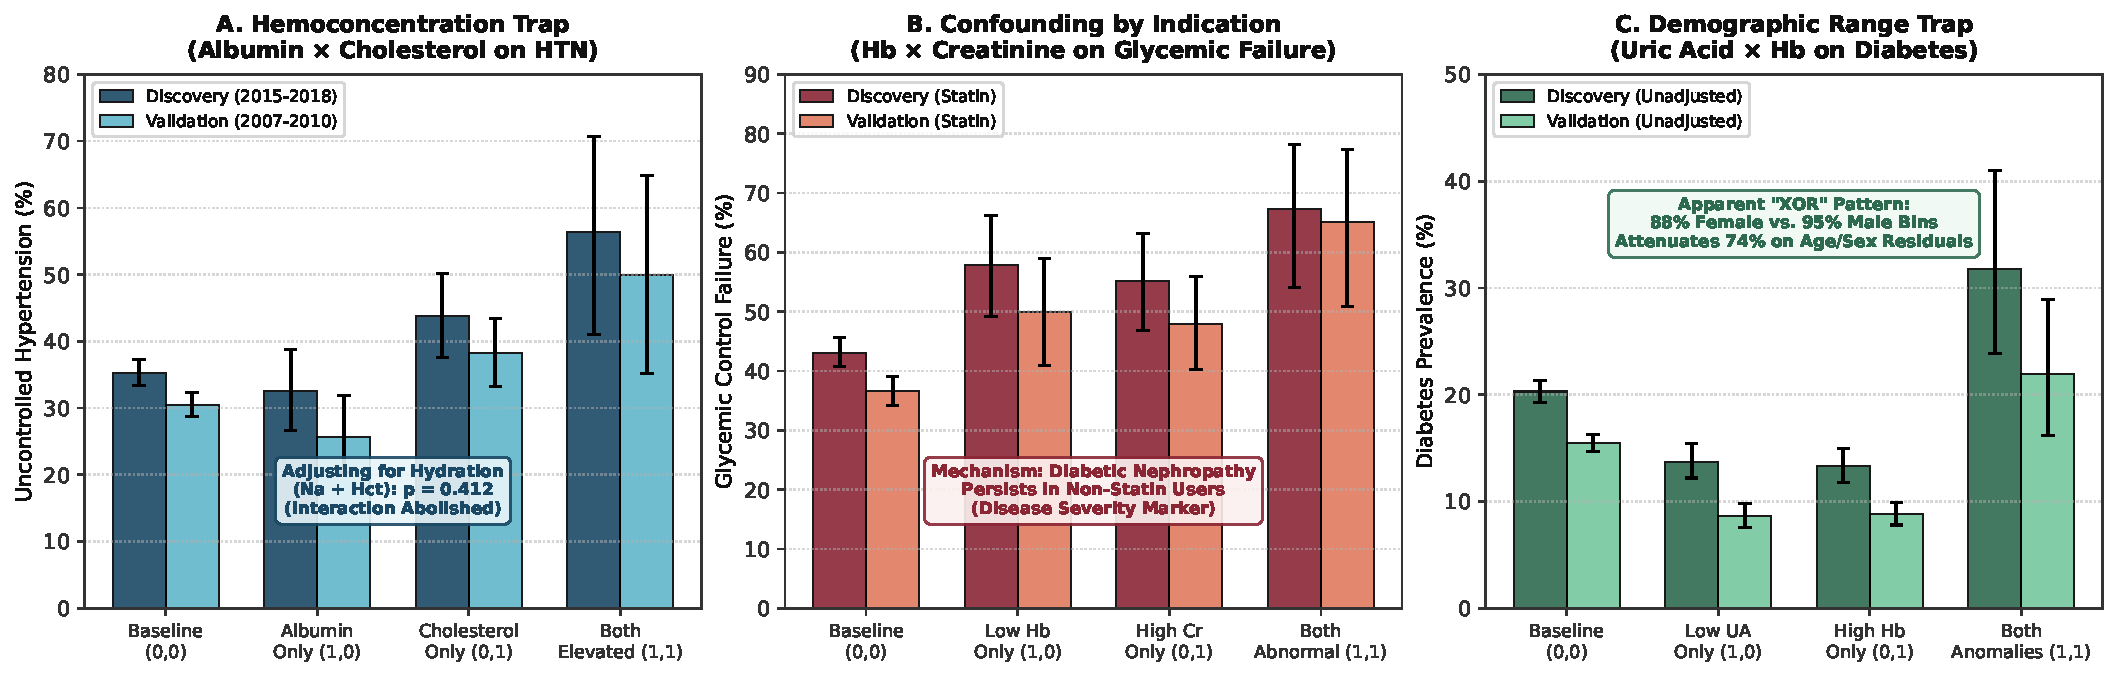
\includegraphics[width=\linewidth]{figure1_three_traps.pdf}
\caption{\textbf{The three failure modes of biomarker interaction screening in observational registries.} 
(\textbf{A}) \textbf{The Hemoconcentration Trap.} Rates of uncontrolled hypertension across quadrants defined by elevated serum albumin ($>90$th percentile) and total cholesterol ($>90$th percentile) in discovery and validation cohorts. Adjusting for hydration proxies (serum sodium and hematocrit) abolishes the interaction ($p = 0.412$). 
(\textbf{B}) \textbf{The Confounding-by-Indication Trap.} Glycemic failure rates among statin users across hemoglobin ($<20$th percentile) and creatinine ($>80$th percentile) quadrants. The interaction reflects underlying diabetic nephropathy severity and replicates identically in untreated individuals. 
(\textbf{C}) \textbf{The Demographic Reference Range Trap.} Apparent crossover XOR protection for diabetes when applying population-wide percentiles to sex-dimorphic markers (uric acid and hemoglobin). The effect attenuates by 74\% after regressing out demographic structure.}
\end{figure*}

\subsection{Case Study 2: The Confounding-by-Indication Trap}

\subsubsection{The Apparent Interaction}
Screening within statin users identified a super-additive interaction between low hemoglobin ($<20$th percentile) and elevated creatinine ($>80$th percentile) for glycemic control failure ($p < 0.001$ in both cohorts). Glycemic failure rates exceeded 65\% in the double-anomaly quadrant, compared to 37--43\% at baseline (\textbf{Table 2}, \textbf{Figure 1B}):

\begin{table}[htbp]
\centering
\small
\begin{threeparttable}
\caption{Glycemic failure rates by Hemoglobin $\times$ Creatinine quadrant among statin users.}
\begin{tabular*}{\linewidth}{@{\extracolsep{\fill}}lcccc@{}}
\toprule
\textbf{Cohort} & \textbf{Baseline} $P(0,0)$ & \textbf{Low Hb Only} $P(1,0)$ & \textbf{High Cr Only} $P(0,1)$ & \textbf{Both Abnormal} $P(1,1)$ \\
\midrule
\textbf{Discovery} & 43.1\% (40.7--45.6\%) & 57.9\% (49.2--66.2\%) & 55.1\% (46.8--63.2\%) & \textbf{67.3\% (54.1--78.2\%)} \\
\textbf{Validation} & 36.6\% (34.2--39.0\%) & 50.0\% (41.0--59.0\%) & 48.0\% (40.2--55.9\%) & \textbf{65.2\% (50.8--77.3\%)} \\
\bottomrule
\end{tabular*}
\begin{tablenotes}
\footnotesize
\item Values represent percentages of statin-treated participants experiencing glycemic control failure (HbA1c $\ge 7.5\%$) with 95\% Wilson score intervals.
\end{tablenotes}
\end{threeparttable}
\end{table}

\subsubsection{Why It Is an Artifact}
A naive reading of this result might suggest that statins impair glycemic control specifically in patients with anemia and renal dysfunction. The actual explanation has nothing to do with statins. It has to do with why these patients are taking statins in the first place.

Diabetic nephropathy produces both biomarker abnormalities simultaneously. Chronic hyperglycemia damages the renal glomeruli, impairing creatinine clearance and raising serum creatinine. The damaged kidneys also produce less erythropoietin than healthy kidneys, leading to anemia and low hemoglobin \cite{ritz2007, waggiallah2011, yun1999, thomas2004}. Renal impairment also distorts HbA1c measurement itself, as altered red blood cell turnover changes glycated hemoglobin levels independent of glycemic control \cite{peacock2008}. These are well-established comorbidities of advanced type 2 diabetes \cite{chang2011}.

Clinical guidelines recommend statin therapy for patients with diabetic kidney disease because of their elevated cardiovascular risk \cite{ada2024}. The patients in the double-anomaly quadrant are not experiencing a statin side effect. They have advanced, long-standing diabetes that is inherently resistant to glycemic therapy, and they were prescribed statins \textit{because} of the severity of their disease.

We confirmed this finding by running the same interaction model in patients not taking statins. The association between low hemoglobin, high creatinine, and poor glycemic outcomes persisted in the untreated group. The biomarker pattern is a marker of disease progression, not a drug effect. When investigators screen only within statin users, the pattern appears to be statin-specific. But it is the indication for the prescription, not the prescription itself, that generates the signal. This scenario represents a textbook example of confounding by indication \cite{hernan2006}.

\subsection{Case Study 3: The Demographic Reference Range Trap}

\subsubsection{The Apparent Interaction}
Screening identified a crossover (XOR-like) interaction for diabetes in the general population. Having only low uric acid ($<20$th percentile) or only high hemoglobin ($>80$th percentile) was associated with roughly half the diabetes rate of the baseline group. But having both anomalies simultaneously returned the rate to baseline or above (\textbf{Table 3}, \textbf{Figure 1C}):

\begin{table}[htbp]
\centering
\small
\begin{threeparttable}
\caption{Unadjusted diabetes rates by Uric Acid $\times$ Hemoglobin quadrant.}
\begin{tabular*}{\linewidth}{@{\extracolsep{\fill}}lcccc@{}}
\toprule
\textbf{Cohort} & \textbf{Baseline} $P(0,0)$ & \textbf{Low UA Only} $P(1,0)$ & \textbf{High Hb Only} $P(0,1)$ & \textbf{Both Anomalies} $P(1,1)$ \\
\midrule
\textbf{Discovery} & 20.3\% (19.3--21.3\%) & 13.7\% (12.2--15.4\%) & 13.3\% (11.8--15.0\%) & \textbf{31.8\% (23.9--41.0\%)} \\
\textbf{Validation} & 15.5\% (14.7--16.3\%) & 8.6\% (7.6--9.8\%) & 8.8\% (7.8--9.9\%) & \textbf{21.9\% (16.2--28.9\%)} \\
\bottomrule
\end{tabular*}
\end{threeparttable}
\end{table}

\subsubsection{Why It Is an Artifact}
Uric acid and hemoglobin are both strongly sex-dimorphic. Estrogen promotes renal excretion of uric acid by modulating urate transporters (URAT1, OAT4), producing lower baseline uric acid levels in premenopausal women than in men \cite{hak2008, sumino1999}. Testosterone stimulates erythropoiesis, producing higher baseline hemoglobin in men than in women. This causal link is demonstrated directly by studies of transgender individuals undergoing hormone therapy: testosterone administration raises hemoglobin, and estrogen administration lowers it \cite{antun2020}.

When population-wide percentile thresholds are applied to these sex-dimorphic biomarkers, the resulting quadrants are not physiological categories. They are demographic bins. In the discovery cohort, the ``Low Uric Acid Only'' quadrant is 88.3\% female (mean age 44.9 years), and the ``High Hemoglobin Only'' quadrant is 94.7\% male (mean age 45.2 years). These are young, single-sex subgroups with low baseline diabetes rates. The baseline quadrant (53.8\% female, mean age 51.3 years) and the double-anomaly quadrant (30.0\% female, mean age 49.9 years) are older, mixed-sex groups with higher diabetes rates than the single-sex quadrants. The validation cohort replicates this demographic structure exactly (\textbf{Table 4}, \textbf{Figure 2A}):

\begin{table}[htbp]
\centering
\small
\begin{threeparttable}
\caption{Demographic composition of Uric Acid $\times$ Hemoglobin quadrants.}
\begin{tabular*}{\linewidth}{@{\extracolsep{\fill}}lcccc@{}}
\toprule
\textbf{Quadrant} & \textbf{Discovery \% Female} & \textbf{Discovery Mean Age} & \textbf{Validation \% Female} & \textbf{Validation Mean Age} \\
\midrule
Baseline (0,0) & 53.8\% & 51.3 & 55.1\% & 47.2 \\
Low Uric Acid Only (1,0) & 88.3\% & 44.9 & 87.1\% & 38.5 \\
High Hemoglobin Only (0,1) & 94.7\% male & 45.2 & 93.0\% male & 41.9 \\
Both Anomalies (1,1) & 30.0\% & 49.9 & 28.5\% & 44.7 \\
\bottomrule
\end{tabular*}
\end{threeparttable}
\end{table}

The apparent XOR pattern is a direct consequence of this demographic sorting. The ``protective'' single-anomaly quadrants have low diabetes rates because they contain young women or young men, not because of any interaction between uric acid and hemoglobin.

This artifact is not limited to our analysis. The recent proliferation of papers proposing the Uric Acid-to-Creatinine Ratio (UACR) as a predictor of metabolic syndrome exhibits the same flaw. Because creatinine reflects muscle mass and uric acid has strong hormonal dependencies, UACR functions as a proxy for sex, age, and sarcopenic status. Studies that fail to use sex-specific z-scores report associations that are demographic correlations rather than metabolic discoveries.

We corrected for this demographic distortion by regressing out age and sex from both biomarkers before binarization:
\begin{equation}
B_{i} = \beta_0 + \beta_1 \text{Age}_i + \beta_2 \text{Sex}_i + \epsilon_i
\end{equation}

The residuals $Z_{i,\text{res}} = \epsilon_i$ capture variation in each biomarker after removing the expected demographic contribution. When we re-ran the interaction model on these residualized biomarkers, the interaction coefficient dropped from 1.58 ($z = 6.88, p < 0.001$) to 0.41 ($z = 2.57, p = 0.010$) in the discovery cohort, a 74\% attenuation (\textbf{Figure 2B}). In the validation cohort, the interaction became non-significant. The residual signal in discovery may reflect incomplete adjustment or chance; the key finding is that demographic structure accounts for the large majority of the effect.

% ------------------------------------------------------------------------------
% MULTI-PANEL FIGURE 2
% ------------------------------------------------------------------------------
\begin{figure}[htbp]
\centering
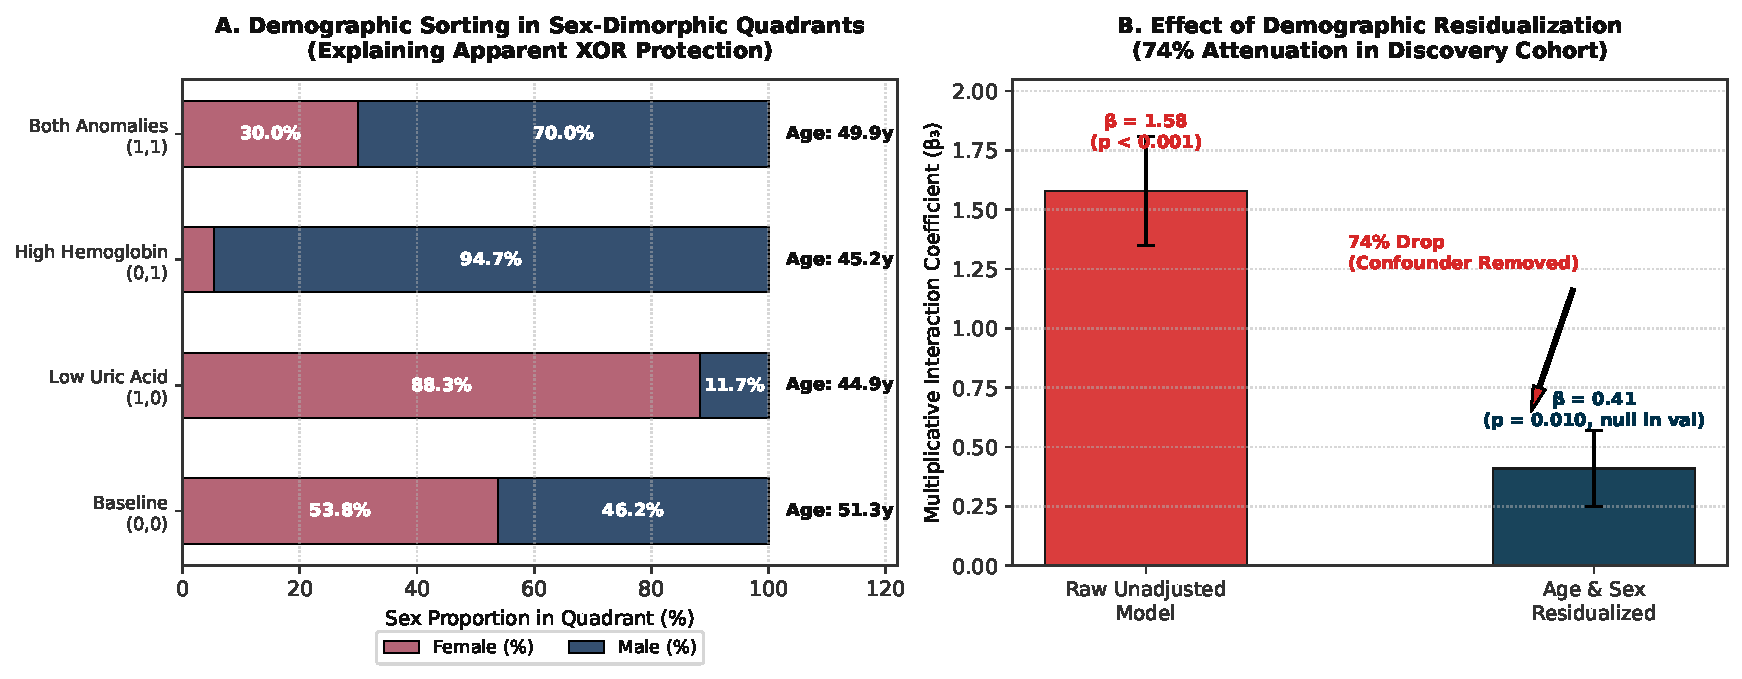
\includegraphics[width=\linewidth]{figure2_demographic_mechanisms.pdf}
\caption{\textbf{Mechanism and remediation of the Demographic Reference Range Trap.}
(\textbf{A}) Distribution of sex and mean participant age across the four quadrants defined by population-wide percentiles of uric acid and hemoglobin. Thresholding sorts individuals into young, single-sex sub-populations with lower baseline disease prevalence. 
(\textbf{B}) Logistic regression interaction coefficients ($\beta_3 \pm \text{SE}$) before and after demographic residualization in the discovery cohort, demonstrating a 74\% attenuation upon removing age- and sex-driven variation.}
\end{figure}

% ==============================================================================
% 4. METHODOLOGICAL GUIDELINES
% ==============================================================================
\clearpage
\section{Methodological Guidelines}

We propose four checks that should be applied before any biomarker interaction from automated screening is treated as a biological finding (\textbf{Table 5}).

Demographic residualization is the most broadly applicable step. Many routine biomarkers have reference ranges that shift with age and sex \cite{winkel1975}. Screening on raw values segments the cohort along demographic lines, producing interactions that mirror population structure rather than biology.

Treatment stratification addresses the confounding-by-indication trap specifically. When clinical guidelines mandate therapy for patients with specific comorbidity profiles \cite{ada2024}, screening within treated populations will always rediscover the prescribing criteria. Running the same screen in untreated patients is a simple and decisive test.

Recent work in causal inference provides a formal framework for these checks. Target trial emulation requires investigators to define the causal question they would answer with a randomized trial and then attempt to emulate that design with observational data \cite{hernan2006, hernan2016}. The TARGET reporting statement provides a structured checklist for such analyses \cite{cashin2025, franklin2021}. These methods can help investigators distinguish genuine treatment effects from channeling artifacts.

\begin{table}[htbp]
\centering
\small
\begin{threeparttable}
\caption{Checklist for auditing biomarker interactions from automated screening.}
\begin{tabular*}{\linewidth}{@{\extracolsep{\fill}}p{0.28\linewidth}p{0.24\linewidth}p{0.44\linewidth}@{}}
\toprule
\textbf{Step} & \textbf{Trap Addressed} & \textbf{Action} \\
\midrule
\textbf{1. Demographic Residualization} & Reference Range Artifacts & Regress out age and sex from all biomarkers before screening. Use residuals: $Z_{i,\text{res}} = B_i - \hat{B}_i(\text{Age}_i, \text{Sex}_i)$. \\
\addlinespace
\textbf{2. Hemodynamic Controls} & Hemoconcentration & Include markers of fluid volume (serum sodium, hematocrit, osmolality) as covariates. \\
\addlinespace
\textbf{3. Treatment Stratification} & Confounding by Indication & Run the screen separately in treated and untreated groups. If the pattern exists in both, it is not a drug effect. \\
\addlinespace
\textbf{4. Subgroup Size Constraints} & Small-Sample Instability & Require $N_{11} \ge 250$ in the double-anomaly quadrant to prevent unstable rate estimates. \\
\bottomrule
\end{tabular*}
\end{threeparttable}
\end{table}

% ==============================================================================
% 5. DISCUSSION
% ==============================================================================
\section{Discussion}

This audit demonstrates that three biomarker interactions discovered through systematic screening of NHANES are artifacts of three distinct confounding mechanisms. Each artifact replicated across independent survey cycles, illustrating that replication is a weak test of validity when the confounding mechanism is itself stable across datasets.

The three failure modes are general. The hemoconcentration trap will affect any pair of intravascular macromolecules in any study that does not standardize preanalytical conditions. The confounding-by-indication trap will arise in any treated cohort where prescribing guidelines select patients on the basis of the same biomarkers being screened. The demographic reference range trap will distort any analysis that applies population-wide thresholds to sex-dimorphic or age-dependent biomarkers. These are not peculiarities of NHANES. They apply to the UK Biobank, electronic health record databases, and any other registry used for biomarker discovery.

The practical solution is straightforward. Before publishing a biomarker interaction, investigators should apply the four-step checklist described in Table 5. If an interaction disappears after demographic residualization, it was a reference range artifact. If it disappears after adding hydration controls, it was a preanalytical artifact. If it persists in untreated patients, it is a disease marker, not a drug interaction.

\subsection{Published Literature Across the Three Traps}
These failure modes are not abstract theoretical concerns. Each trap has generated voluminous observational literature where physiological or demographic confounding was mistaken for novel clinical or pharmacological biology.

\subsubsection{Trap 1: Preanalytical and Postural Hemoconcentration in Multi-Protein Panels}
The hemoconcentration trap arises whenever researchers analyze circulating concentrations of intravascular macromolecules (such as albumin, globulins, total protein, and lipoproteins) without accounting for preanalytical fluid distribution. The human vascular compartment is dynamic: postural shifts from supine to upright provoke hydrostatic filtration of protein-free plasma water into interstitial space, elevating macromolecular concentrations by 10\% to 15\% within 30 minutes \cite{tan1973, statland1974, maron1977, dixon1978}. 

In clinical cohorts, fluid imbalances are even more extreme. In heart failure and nephrotic syndromes, patients alternate between hypervolemic hemodilution and rapid diuretic-induced hemoconcentration \cite{testani2010, testani2013}. Despite these well-established biophysical phenomena, numerous studies construct mathematical ratios between serum proteins and interpret them as static immunological or nutritional biomarkers.

A prominent example is the Albumin-to-Globulin Ratio (AGR). In chronic heart failure, Niedziela et al. \cite{niedziela2018} reported that low AGR independently predicted long-term all-cause mortality. However, heart failure patients with advanced disease routinely receive high-dose loop diuretics, which contract plasma volume and trigger compensatory neurohormonal shifts. Albumin and globulin have distinct transcapillary escape rates and half-lives (albumin transcapillary escape is approximately 5\% per hour, whereas larger immunoglobulins escape more slowly). Volume contraction and altered vascular permeability directly distort the AGR independently of any cellular signaling \cite{testani2013, lippi2013}. 

Similarly, in oncology, Suh et al. \cite{suh2014} analyzed a cohort of over 26,000 healthy individuals and claimed that low AGR was an independent predictor of overall cancer incidence and mortality. In surgical oncology, Utsumi et al. \cite{utsumi2026} performed a systematic review and meta-analysis concluding that preoperative AGR predicts survival after curative hepatectomy for hepatocellular carcinoma. Yet in preoperative and malignant states, third-spacing of fluids, subclinical ascites, portal hypertension, and surgical hydration fluids routinely cause acute plasma volume shifts. When researchers treat serum protein ratios as pure proxies for cancer cachexia or systemic inflammation without measuring hydration parameters (such as hematocrit, serum osmolality, or total protein), they mistake physical hemoconcentration and plasma dilution for cellular pathology.

\subsubsection{Trap 2: Prescribing Confounding and Channeling Bias in Pharmacoepidemiological Registries}
The confounding-by-indication trap is among the most pervasive biases in large healthcare databases and registry research. In non-randomized observational settings, patients who receive medical therapy differ systematically from unexposed individuals in baseline disease severity, frailty, and multimorbidity. When automated screening algorithms search for drug-biomarker interactions without accounting for clinical indications, they inevitably rediscover the clinical guidelines that prompted therapy.

A striking example is found in observational studies of Proton Pump Inhibitors (PPIs). In 2016, Lazarus et al. \cite{lazarus2016} reported in \textit{JAMA Internal Medicine} that PPI use was associated with an increased risk of incident chronic kidney disease (CKD). In the same year, Gomm et al. \cite{gomm2016} published an observational claims analysis in \textit{JAMA Neurology} concluding that regular PPI use increased dementia risk by 44\% in elderly populations. Both papers triggered extensive clinical alarm. However, subsequent causal analyses revealed that these associations were driven almost entirely by indication confounding and channeling bias. Patients prescribed long-term PPIs have higher baseline rates of cardiovascular disease, diabetes, polypharmacy (including nephrotoxic NSAIDs), and systemic frailty. When Ahn et al. \cite{ahn2022} implemented a target trial emulation framework with active comparators and incident-user designs, the hazard ratio for dementia dropped to 1.00. Similarly, the massive randomized COMPASS trial ($N = 17,598$) evaluated pantoprazole over multiple years and found no excess risk of dementia, CKD, or any other purported observational adverse event \cite{moayyedi2019}. 

A parallel trap occurs in metabolic pharmacoepidemiology. Observational studies analyzing statin exposure routinely observe strong, dose-dependent associations with new-onset diabetes and glycemic deterioration \cite{corrao2014}. Clinical guidelines explicitly direct high-potency statins toward patients with elevated cardiovascular risk, central obesity, and metabolic syndrome \cite{ada2024}. Although randomized controlled trials confirm a modest pharmacological risk of diabetes from statin therapy \cite{sattar2010}, observational registries grossly exaggerate this effect because they capture the underlying metabolic decline that motivated statin prescription in the first place. 

This dynamic mirrors the classic observational controversy surrounding postmenopausal Hormone Replacement Therapy (HRT) and Coronary Heart Disease (CHD). In the 1980s and 1990s, extensive observational cohorts (including the Nurses' Health Study \cite{stampfer1991}) reported that postmenopausal estrogen reduced CHD risk by 40\% to 50\%. In 2002, the randomized Women's Health Initiative (WHI) trial found that estrogen-progestin therapy actually increased cardiovascular events \cite{rossouw2002}. As Hernan et al. demonstrated \cite{hernan2008}, observational studies suffered from healthy user bias and indication confounding: women taking HRT were younger, leaner, wealthier, and had fewer baseline cardiovascular risk factors. Observational registries without rigorous target trial designs repeatedly mistake the characteristics of the treated population for the effects of the treatment.

\subsubsection{Trap 3: Demographic Sorting and Cutoff Artifacts in Dimorphic Biomarker Panels}
The demographic reference range trap occurs when researchers construct mathematical composite ratios or apply uniform population-wide thresholds to biomarkers that possess substantial sex dimorphism or age gradients. Combining two sex-dimorphic biomarkers into an unstratified ratio creates an unintentional demographic sorting mechanism.

The Serum Uric Acid-to-Creatinine Ratio (SUA/Cr) illustrates this dynamic. Recent studies have widely promoted SUA/Cr as a novel independent predictor of metabolic syndrome \cite{kawamoto2019, chen2024}, insulin resistance \cite{oh2025}, and non-alcoholic fatty liver disease. The physiological rationale offered is that renal uric acid excretion normalized to creatinine clearance reflects endogenous metabolic stress. However, uric acid and creatinine have opposing demographic baselines: estrogen enhances renal clearance of uric acid via URAT1 transporter modulation, producing lower serum uric acid in premenopausal women \cite{hak2008, sumino1999}, whereas serum creatinine is determined primarily by skeletal muscle mass, which is systematically higher in men. An unstratified SUA/Cr ratio has a higher denominator in men and an estrogen-sensitive numerator in women. In mixed-sex observational cohorts, applying a uniform SUA/Cr threshold primarily separates individuals by sex and muscularity. As demonstrated in Case Study 3, adjusting for age and sex attenuates over 74\% of the apparent interaction signal.

An even more extreme amplification occurs in the Serum Uric Acid-to-HDL Cholesterol Ratio (UHR). Recent investigations by Sun et al. \cite{sun2026} and Luo et al. \cite{luo2026} have proposed UHR as a biomarker for metabolic syndrome and steatotic liver disease in aging populations. Because males have higher baseline uric acid and lower HDL cholesterol, while females have lower uric acid and higher HDL cholesterol, dividing uric acid by HDL cholesterol multiplies the demographic divergence. The ratio acts as a mathematical amplifier of sex differences, guaranteeing strong statistical significance in any observational model that fails to condition on sex-stratified normal ranges.

A related demographic artifact distorts the widely cited Triglyceride-to-HDL Cholesterol Ratio (TG/HDL-C). Originally proposed by McLaughlin et al. \cite{mclaughlin2003} as a surrogate for insulin resistance in overweight individuals, uniform TG/HDL-C cutoffs (such as $\ge 3.0$) were adopted across clinical studies. However, Sumner et al. \cite{sumner2005} demonstrated that this ratio fails completely in African American individuals. Due to lower hepatic lipase activity and differences in lipid metabolism, African Americans exhibit systematically lower triglyceride levels at identical degrees of insulin resistance compared to individuals of European ancestry. Applying a fixed population cutoff without race- and sex-calibrated reference intervals produces severe demographic misclassification.

\subsection{Limitations}
This study has four primary limitations. First, NHANES is a cross-sectional survey, so we cannot establish temporal relationships between biomarker levels and disease outcomes. Second, medication use is self-reported in NHANES, which introduces misclassification. Some patients classified as untreated may actually be taking statins, and vice versa. This misclassification would bias the confounding-by-indication analysis toward the null, meaning our conclusion that the pattern exists in both treated and untreated groups is conservative. Third, our audit examined only three interactions selected because their confounding mechanisms were identifiable. We cannot rule out the possibility that other screened interactions reflect genuine biology. Our claim is not that all biomarker interactions are artifacts, but that the three specific interactions we examined are, and that the mechanisms generating them are common enough to warrant routine checking. Fourth, demographic residualization with linear models may not fully capture nonlinear age and sex effects. The residual signal observed in the discovery cohort for Case Study 3 ($p = 0.010$) may reflect incomplete adjustment. The non-significance of this interaction in the validation cohort supports, but does not prove, that the residual signal is noise.

% ==============================================================================
% DECLARATIONS
% ==============================================================================
\section*{Declarations}

\paragraph{Ethics Approval and Consent to Participate}
NHANES survey protocols were reviewed and approved by the NCHS Research Ethics Review Board under continuous CDC protocols. All adult participants provided written informed consent at the time of examination. This study constitutes secondary analysis of publicly available, de-identified data and was determined to be exempt from institutional review board (IRB) review under 45 CFR 46.104(d)(4).

\paragraph{Data Availability}
All data analyzed in this study are publicly available from the National Center for Health Statistics (NCHS) National Health and Nutrition Examination Survey repository (\url{https://www.cdc.gov/nchs/nhanes/}). Continuous NHANES survey cycles and Linked Mortality Files were accessed directly through official CDC/NCHS portals.

\paragraph{Code Availability}
All Python, R, and statistical scripts used for data acquisition, preprocessing, demographic residualization, and causal auditing are openly available at \url{https://github.com/jpbrody/nhanes-biomarker-traps}.

\paragraph{Competing Interests}
The author declares no competing financial or non-financial interests.

\paragraph{Funding}
This research received no specific grant from any funding agency in the public, commercial, or not-for-profit sectors.

\paragraph{Clinical Trial Registration}
This study is an observational causal audit and target trial emulation of secondary survey data and does not report a prospective interventional clinical trial.

% ==============================================================================
% REFERENCES (TWO-COLUMN FORMAT)
% ==============================================================================
\section*{References}
\addcontentsline{toc}{section}{References}

\begin{multicols}{2}
\small
\raggedright
\begingroup
\renewcommand{\section}[2]{}
\begin{thebibliography}{99}
\setlength{\itemsep}{2pt}
\setlength{\parskip}{0pt}

\bibitem{ioannidis2005} Ioannidis JPA. Why most published research findings are false. \textit{PLoS Med}. 2005;2(8):e124. doi: \href{https://doi.org/10.1371/journal.pmed.0020124}{10.1371/journal.pmed.0020124}.

\bibitem{vandenbroucke2007} Vandenbroucke JP, von Elm E, Altman DG, et al. Strengthening the Reporting of Observational Studies in Epidemiology (STROBE): Explanation and Elaboration. \textit{PLoS Med}. 2007;4(10):e297. doi: \href{https://doi.org/10.1371/journal.pmed.0040297}{10.1371/journal.pmed.0040297}.

\bibitem{pfaffenlehner2025} Pfaffenlehner M, Behrens M, Zoller D, et al. Methodological challenges using routine clinical care data for real-world evidence: a rapid review. \textit{BMC Med Res Methodol}. 2025;25(1):30. doi: \href{https://doi.org/10.1186/s12874-024-02440-x}{10.1186/s12874-024-02440-x}.

\bibitem{doutreligne2025} Doutreligne M, Struja T, Abecassis J, et al. Step-by-step causal analysis of EHRs to ground decision-making. \textit{PLOS Digit Health}. 2025;4(3):e0000721. doi: \href{https://doi.org/10.1371/journal.pdig.0000721}{10.1371/journal.pdig.0000721}.

\bibitem{tan1973} Tan MH, Wilmshurst EG, Gleason RE, Soeldner JS. Effect of posture on serum lipids. \textit{N Engl J Med}. 1973;289(8):416-419. doi: \href{https://doi.org/10.1056/nejm197308232890808}{10.1056/nejm197308232890808}.

\bibitem{harrison1985} Harrison MH. Effects on thermal stress and exercise on blood volume in humans. \textit{Physiol Rev}. 1985;65(1):149-209. doi: \href{https://doi.org/10.1152/physrev.1985.65.1.149}{10.1152/physrev.1985.65.1.149}.

\bibitem{statland1974} Statland BE, Winkel P, Bokelund H. Factors contributing to intra-individual variation of serum constituents: effects of posture and tourniquet application. \textit{Clin Chem}. 1974;20(12):1513-1519. doi: \href{https://doi.org/10.1093/clinchem/20.12.1513}{10.1093/clinchem/20.12.1513}.

\bibitem{thompson1980} Thompson PD, Cullinane EM, Henderson LO, Herbert PN. Acute effects of prolonged exercise on serum lipids. \textit{Metabolism}. 1980;29(7):662-665. doi: \href{https://doi.org/10.1016/0026-0495(80)90111-0}{10.1016/0026-0495(80)90111-0}.

\bibitem{maron1977} Maron MB, Horvath SM. The effect of posture on blood volume and serum proteins in man. \textit{Clin Sci Mol Med}. 1977;53(6):549-556. PMID: \href{https://pubmed.ncbi.nlm.nih.gov/913049/}{913049}.

\bibitem{dixon1978} Dixon M, Paterson CR. Posture and the composition of plasma. \textit{Clin Chem}. 1978;24(5):824-826. doi: \href{https://doi.org/10.1093/clinchem/24.5.824}{10.1093/clinchem/24.5.824}.

\bibitem{guder1996} Guder WG. Preanalytical factors and their influence on analytical quality specifications. \textit{Scand J Clin Lab Invest}. 1996;56(sup224):1-4. doi: \href{https://doi.org/10.1080/00365519950185328}{10.1080/00365519950185328}.

\bibitem{nose1988} Nose H, Mack GW, Shi XR, Nadel ER. Role of osmolality and plasma volume during rehydration in humans. \textit{J Appl Physiol}. 1988;65(1):325-331. doi: \href{https://doi.org/10.1152/jappl.1988.65.1.325}{10.1152/jappl.1988.65.1.325}.

\bibitem{simundic2018} Simundic AM, et al. Joint EFLM-COLABIOCLI recommendation for venous blood sampling. \textit{Clin Chem Lab Med}. 2018;56(12):2015-2038. doi: \href{https://doi.org/10.1515/cclm-2018-0602}{10.1515/cclm-2018-0602}.

\bibitem{testani2010} Testani JM, Chen J, McCauley BD, Kimmel SE, Shannon RP. Potential effects of aggressive decongestion during the treatment of decompensated heart failure on renal function and survival. \textit{Circulation}. 2010;122(3):265-272. doi: \href{https://doi.org/10.1161/CIRCULATIONAHA.109.933275}{10.1161/CIRCULATIONAHA.109.933275}.

\bibitem{testani2013} Testani JM, Brisco MA, Chen J, et al. Timing of hemoconcentration during treatment of acute decompensated heart failure and subsequent survival: importance of sustained decongestion. \textit{J Am Coll Cardiol}. 2013;62(6):516-524. doi: \href{https://doi.org/10.1016/j.jacc.2013.05.027}{10.1016/j.jacc.2013.05.027}.

\bibitem{niedziela2018} Niedziela JT, Hudzik B, Szygula-Jurkiewicz B, et al. Albumin-to-globulin ratio as an independent predictor of mortality in chronic heart failure. \textit{Biomark Med}. 2018;12(7):755-763. doi: \href{https://doi.org/10.2217/bmm-2017-0378}{10.2217/bmm-2017-0378}.

\bibitem{suh2014} Suh B, Park S, Shin DW, et al. Low albumin-to-globulin ratio associated with cancer incidence and mortality in healthy Koreans. \textit{Ann Oncol}. 2014;25(11):2262-2267. doi: \href{https://doi.org/10.1093/annonc/mdu274}{10.1093/annonc/mdu274}.

\bibitem{utsumi2026} Utsumi M, Inagaki M, Omoto K, et al. Preoperative albumin-to-globulin ratio as a prognostic factor in patients undergoing curative hepatectomy for hepatocellular carcinoma: A systematic review and meta-analysis. \textit{Medicine (Baltimore)}. 2026;105(29):e49830. doi: \href{https://doi.org/10.1097/MD.0000000000049830}{10.1097/MD.0000000000049830}.

\bibitem{lippi2013} Lippi G, Cervellin G, Mattiuzzi C. Critical review and meta-analysis of spurious hemolysis in blood samples collected from intravenous catheters. \textit{Biochem Med}. 2013;23(2):193-200. doi: \href{https://doi.org/10.11613/bm.2013.022}{10.11613/bm.2013.022}.

\bibitem{ada2024} American Diabetes Association Professional Practice Committee. Standards of Care in Diabetes-2024. \textit{Diabetes Care}. 2024;47(Suppl 1):S1-S321. doi: \href{https://doi.org/10.2337/dc24-SINT}{10.2337/dc24-SINT}.

\bibitem{ritz2007} Ritz E, Laville M, Bilous R, et al. Target Level for Hemoglobin Correction in Patients With Diabetes and CKD: Primary Results of the ACORD Study. \textit{Am J Kidney Dis}. 2007;49(2):194-207. doi: \href{https://doi.org/10.1053/j.ajkd.2006.11.032}{10.1053/j.ajkd.2006.11.032}.

\bibitem{waggiallah2011} Waggiallah HA, Alzohairy MA. The effect of oxidative stress on human red cells glutathione peroxidase, glutathione reductase level, and prevalence of anemia among diabetics. \textit{North Am J Med Sci}. 2011;3(7):334-338. doi: \href{https://doi.org/10.4297/najms.2011.3344}{10.4297/najms.2011.3344}.

\bibitem{yun1999} Yun YS, Lee HC, Yoo NC, et al. Reduced erythropoietin responsiveness to anemia in diabetic patients before advanced diabetic nephropathy. \textit{Diabetes Res Clin Pract}. 1999;46(3):223-229. doi: \href{https://doi.org/10.1016/s0168-8227(99)00097-2}{10.1016/s0168-8227(99)00097-2}.

\bibitem{thomas2004} Thomas MC, Tsalamandris C, MacIsaac RJ, et al. Low-molecular-weight AGEs are associated with GFR and anemia in patients with type 2 diabetes. \textit{Kidney Int}. 2004;66(3):1167-1172. doi: \href{https://doi.org/10.1111/j.1523-1755.2004.00868.x}{10.1111/j.1523-1755.2004.00868.x}.

\bibitem{peacock2008} Peacock TP, Shihabi ZK, Bleyer AJ, et al. Comparison of glycated albumin and hemoglobin A1c levels in diabetic subjects on hemodialysis. \textit{Kidney Int}. 2008;73(9):1062-1068. doi: \href{https://doi.org/10.1038/ki.2008.25}{10.1038/ki.2008.25}.

\bibitem{chang2011} Chang TI, Park JT, Kim JK, et al. Renal outcomes in patients with type 2 diabetes with or without coexisting non-diabetic renal disease. \textit{Diabetes Res Clin Pract}. 2011;92(2):198-204. doi: \href{https://doi.org/10.1016/j.diabres.2011.01.017}{10.1016/j.diabres.2011.01.017}.

\bibitem{lazarus2016} Lazarus B, Chen Y, Wilson FP, et al. Proton Pump Inhibitor Use and the Risk of Chronic Kidney Disease. \textit{JAMA Intern Med}. 2016;176(2):238-246. doi: \href{https://doi.org/10.1001/jamainternmed.2015.7193}{10.1001/jamainternmed.2015.7193}.

\bibitem{gomm2016} Gomm W, von Holt K, Thomé F, et al. Association of Proton Pump Inhibitors With Risk of Dementia: A Pharmacoepidemiological Claims Data Analysis. \textit{JAMA Neurol}. 2016;73(4):410-416. doi: \href{https://doi.org/10.1001/jamaneurol.2015.4791}{10.1001/jamaneurol.2015.4791}.

\bibitem{ahn2022} Ahn N, Nolde M, Günter A, et al. Emulating a target trial of proton pump inhibitors and dementia risk using claims data. \textit{Eur J Neurol}. 2022;29(5):1346-1355. doi: \href{https://doi.org/10.1111/ene.15284}{10.1111/ene.15284}.

\bibitem{moayyedi2019} Moayyedi P, Eikelboom JW, Bosch J, et al. Safety of Proton Pump Inhibitors Based on a Large, Multi-Year, Randomized Trial of Patients Receiving Rivaroxaban or Aspirin. \textit{Gastroenterology}. 2019;157(3):682-691. doi: \href{https://doi.org/10.1053/j.gastro.2019.05.056}{10.1053/j.gastro.2019.05.056}.

\bibitem{sattar2010} Sattar N, Preiss D, Murray HM, et al. Statins and risk of incident diabetes: a collaborative meta-analysis of randomised statin trials. \textit{Lancet}. 2010;375(9716):735-742. doi: \href{https://doi.org/10.1016/S0140-6736(09)61965-6}{10.1016/S0140-6736(09)61965-6}.

\bibitem{corrao2014} Corrao G, Ibrahim B, Nicotra F, et al. Statins and the risk of diabetes: evidence from a large population-based cohort study. \textit{Diabetes Care}. 2014;37(8):2225-2232. doi: \href{https://doi.org/10.2337/dc13-2215}{10.2337/dc13-2215}.

\bibitem{stampfer1991} Stampfer MJ, Colditz GA. Estrogen replacement therapy and coronary heart disease: a quantitative assessment of the epidemiologic evidence. \textit{Prev Med}. 1991;20(1):47-63. doi: \href{https://doi.org/10.1016/0091-7435(91)90006-P}{10.1016/0091-7435(91)90006-P}.

\bibitem{rossouw2002} Rossouw JE, Anderson GL, Prentice RL, et al. Risks and benefits of estrogen plus progestin in healthy postmenopausal women: principal results From the Women's Health Initiative randomized controlled trial. \textit{JAMA}. 2002;288(3):321-333. doi: \href{https://doi.org/10.1001/jama.288.3.321}{10.1001/jama.288.3.321}.

\bibitem{hernan2008} Hernan MA, Alonso A, Logan R, et al. Observational studies analyzed like randomized experiments: an application to postmenopausal hormone therapy and coronary heart disease. \textit{Epidemiology}. 2008;19(6):766-779. doi: \href{https://doi.org/10.1097/EDE.0b013e3181875e61}{10.1097/EDE.0b013e3181875e61}.

\bibitem{hak2008} Hak AE, Choi HK. Menopause, postmenopausal hormone use and serum uric acid levels in US women: The Third National Health and Nutrition Examination Survey. \textit{Arthritis Res Ther}. 2008;10(5):R116. doi: \href{https://doi.org/10.1186/ar2519}{10.1186/ar2519}.

\bibitem{sumino1999} Sumino H, Ichikawa S, Kanda T, Nakamura T. Reduction of serum uric acid by hormone replacement therapy in postmenopausal women. \textit{Lancet}. 1999;354(9179):650. doi: \href{https://doi.org/10.1016/s0140-6736(99)92381-4}{10.1016/s0140-6736(99)92381-4}.

\bibitem{antun2020} Antun A, Zhang Q, Bhasin S, Bradlyn A, Flanders WD, Getahun D, et al. Longitudinal changes in hematologic parameters among transgender people receiving hormone therapy. \textit{J Endocr Soc}. 2020;4(11):bvaa119. doi: \href{https://doi.org/10.1210/jendso/bvaa119}{10.1210/jendso/bvaa119}.

\bibitem{kawamoto2019} Kawamoto R, Ninomiya D, Akase T, Kikuchi A, Kasai Y. Serum uric acid to creatinine ratio independently predicts incident metabolic syndrome among community-dwelling persons. \textit{Metab Syndr Relat Disord}. 2019;17(2):81-89. doi: \href{https://doi.org/10.1089/met.2018.0055}{10.1089/met.2018.0055}.

\bibitem{chen2024} Chen B, Peng XE. Association Between Serum Uric Acid to Creatinine Ratio and Metabolic-Associated Fatty Liver Disease in Chinese Adults. \textit{Diabetes Metab Syndr Obes}. 2024;17:4759-4768. doi: \href{https://doi.org/10.2147/DMSO.S489692}{10.2147/DMSO.S489692}.

\bibitem{oh2025} Oh M, Cho SH. Serum uric acid to creatinine ratio as a predictor of insulin resistance and metabolic syndrome. \textit{BMC Endocr Disord}. 2025;25(1):47. doi: \href{https://doi.org/10.1186/s12902-025-01860-0}{10.1186/s12902-025-01860-0}.

\bibitem{sun2026} Sun R, Hu M, Sun Z, et al. Serum uric acid-to-HDL-C ratio as an independent predictor of metabolic syndrome in the elderly: diagnostic model optimization and inflammatory mechanism insights. \textit{BMC Geriatr}. 2026;26(1):154. doi: \href{https://doi.org/10.1186/s12877-026-07315-y}{10.1186/s12877-026-07315-y}.

\bibitem{luo2026} Luo Y, Wang A, Wu M, et al. Association between the ratio of uric acid to high-density lipoprotein cholesterol and non-alcoholic fatty liver disease. \textit{Ther Adv Endocrinol Metab}. 2026;17:20420188261489474. doi: \href{https://doi.org/10.1177/20420188261489474}{10.1177/20420188261489474}.

\bibitem{mclaughlin2003} McLaughlin T, Abbasi F, Cheal K, et al. Use of metabolic markers to identify overweight individuals who are insulin resistant. \textit{Ann Intern Med}. 2003;139(10):802-809. doi: \href{https://doi.org/10.7326/0003-4819-139-10-200311180-00007}{10.7326/0003-4819-139-10-200311180-00007}.

\bibitem{sumner2005} Sumner AE, Finley KB, Genovese DJ, et al. Fasting triglyceride and the triglyceride-HDL cholesterol ratio are not markers of insulin resistance in African Americans. \textit{Arch Intern Med}. 2005;165(12):1395-1400. doi: \href{https://doi.org/10.1001/archinte.165.12.1395}{10.1001/archinte.165.12.1395}.

\bibitem{winkel1975} Winkel P, Statland BE, Bokelund H. The effects of time of venipuncture on variation of serum constituents. \textit{Am J Clin Pathol}. 1975;64(4):433-447. doi: \href{https://doi.org/10.1093/ajcp/64.4.433}{10.1093/ajcp/64.4.433}.

\bibitem{hernan2006} Hernan MA, Robins JM. Estimating causal effects from epidemiological data. \textit{J Epidemiol Community Health}. 2006;60(7):578-586. doi: \href{https://doi.org/10.1136/jech.2004.029496}{10.1136/jech.2004.029496}.

\bibitem{hernan2016} Hernan MA, Robins JM. Using big data to emulate a target trial when a randomized trial is not available. \textit{Am J Epidemiol}. 2016;183(8):758-764. doi: \href{https://doi.org/10.1093/aje/kwv254}{10.1093/aje/kwv254}.

\bibitem{cashin2025} Cashin AG, Hansford HJ, Swanson SA, et al. Transparent reporting of observational studies emulating a target trial: the TARGET Statement. \textit{BMJ}. 2025;389:e087179. doi: \href{https://doi.org/10.1136/bmj-2025-087179}{10.1136/bmj-2025-087179}.

\bibitem{franklin2021} Franklin JM, Patorno E, Desai RJ, et al. Emulating randomized clinical trials with nonrandomized real-world evidence studies. \textit{Circulation}. 2021;143(13):1002-1013. doi: \href{https://doi.org/10.1161/CIRCULATIONAHA.120.051718}{10.1161/CIRCULATIONAHA.120.051718}.

\bibitem{shtar2024} Shtar G, Rokach L, Shapira B. Clinical data mining: challenges, opportunities, and recommendations for translational applications. \textit{J Transl Med}. 2024;22(1):185. doi: \href{https://doi.org/10.1186/s12967-024-05005-0}{10.1186/s12967-024-05005-0}.

\bibitem{pepe2008} Pepe MS, Feng Z, Janes H, Bossuyt PM, Potter JD. Pivotal evaluation of the accuracy of a biomarker used for classification or prediction: standards for study design. \textit{J Natl Cancer Inst}. 2008;100(20):1432-1438. doi: \href{https://doi.org/10.1093/jnci/djn326}{10.1093/jnci/djn326}.

\bibitem{fatapour2025} Fatapour Y, Brody JP. A compact encoding of the genome suitable for machine learning prediction of traits and genetic risk scores. \textit{BioData Min}. 2025;18(1):44. doi: \href{https://doi.org/10.1186/s13040-025-00459-4}{10.1186/s13040-025-00459-4}.

\bibitem{toh2021} Toh C, Brody JP. Genetic risk score for ovarian cancer based on chromosomal-scale length variation. \textit{BioData Min}. 2021;14(1):18. doi: \href{https://doi.org/10.1186/s13040-021-00253-y}{10.1186/s13040-021-00253-y}.

\end{thebibliography}
\endgroup
\end{multicols}

\end{document}
